\documentclass[9pt]{beamer}
% package list
\usepackage{./Amsterdam}
\usepackage{graphicx}
\usepackage[framemethod=TikZ]{mdframed}
\usepackage{wrapfig}
% setting 
\definecolor{MidnightBlue}{RGB}{0,103,149}
\setbeamertemplate{frametitle}{\hspace{-0.5cm}\bf\insertframetitle}
% prensentation info
\title[Application of Conditional Random Fields in Salient Object Detection]
{\bf {Application of Conditional Random Fields in \\Salient Object Detection within an Image,\\using Local, Regional, and Global Features}}
\author[Jimmy Lin and Chris Claoue Long]{\bf Jimmy Lin \\Chris Claoue Long}
\institute{\bf Dr. Stephen Gould\\[0.3cm] College of Engineering and Computer Science \\Australian National University}
\date{\bf \today}
% new command definition
\DeclareMathOperator*{\argmin}{arg\,min}
\DeclareMathOperator*{\argmax}{arg\,max}
\newcommand{\SUM}{\sum\limits}
%%% beginning of document
\begin{document}
\begin{large}
\frame{\begin{mdframed}[roundcorner=10pt]\maketitle\end{mdframed}}%\titlepage}
\end{large}

%{{{ Introduction
\section{Introduction}
\frame{
    \frametitle{Introduction and Motivation}
    \begin{center}
    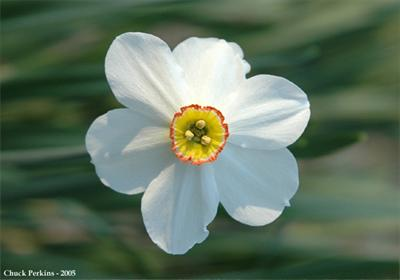
\includegraphics[width=1.6in,height=1.15in]{salientExample/PM1.jpg} \hspace{0.1cm}
    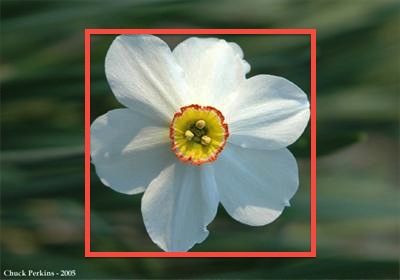
\includegraphics[width=1.6in,height=1.15in]{salientExample/PM.jpg}\\
    {\footnotesize Images from MSRA dataset B}
    \end{center}
    Saliency is the prominence of an object in an image.\\[10pt]  Often detected by its high contrast to its boundary with the background, its unique colour distribution compared to its surrounds, and the break in spatial continuity of colour that it represents in the image.\\[10pt]
    Salient object detection is useful in numerous areas!
}
%}}}

%{{{ Related Works
\section{Related Works}
\frame{
    \frametitle{Related Works}
    \begin{itemize}
        \item Salient-based Model (SM,1998) \\
        \begin{thebibliography}{9}
        \footnotesize
        \bibitem{ConcreteMath} Itti, Laurent, Christof Koch, and Ernst Niebur. "A model of saliency-based visual attention for rapid scene analysis."\textit{ Pattern Analysis and Machine Intelligence, IEEE Transactions on 20.11 (1998): 1254-1259.}
    \end{thebibliography}

    \item Fuzzy Growing Method (FG,2003) \\
        \begin{thebibliography}{9}
            \footnotesize
            \bibitem{ConcreteMath} Ma, Yu-Fei, and Hong-Jiang Zhang. "Contrast-based image attention analysis by using fuzzy growing."\textit{ Proceedings of the eleventh ACM international conference on Multimedia. ACM, 2003.} 
            \end{thebibliography}
    \item CRF-based Model (CRFM,2007)
        \begin{thebibliography}{9}
            \footnotesize 
            \bibitem{ConcreteMath} Liu, Tie, et al. "Learning to detect a salient object."\textit{ Computer Vision and Pattern Recognition, 2007. CVPR'07. IEEE Conference on. IEEE, 2007. }
            \bibitem Liu, Tie, et al. "Learning to detect a salient object."\textit{ Pattern Analysis and Machine Intelligence, IEEE Transactions on 33.2 (2011): 353-367.}
        \end{thebibliography}
    \end{itemize}
PICTURES HERE?
}
%}}}

%{{{ Problem Formulation
\section{Problem Formulation}
\frame{
    {\bf \sectionpage}
    \frametitle{Formulation}
    Given an image $I$, we want to compute the location of a salient object.\\[10pt]
    Binary labelling task -- for each pixel $x$, indicate whether it belongs to the salient object (1) or not (0)\\[10pt]
    Build up a probabilistic model $P(A|I)=\frac{1}{Z}e^{-E(A|I)}$, where $\frac{1}{Z}$ is the normalising factor, and $E(A|I)$ is the energy function incorporating both unary/static and pairwise potentials between pixels.\\[10pt]
    
    
%    calculate the local, regional and global features.\\
%    In our program, we used contrast (local), centre-surround histogram comparisons around potentially salient areas (regional) and the colour spatial distribution of the image (global).\\[10pt] 
%    We then run CRF inference over the outcome of these calculations, and select the region that seems most probable to be salient, effectively a winner-takes-all approach. Finally, we output a bounding box rectangle that encompasses this region.
}
\frame{
    \frametitle{Energy function in more detail}
    $$
    E(A|I) = \SUM_x \SUM_{k=1}^K \lambda_k \cdot F_k(a_x,I) + \SUM_{x,x'}S(a_x,a_{x'},I)
    $$
    where $\lambda_k$ is the weight of the $k^{th}$ feature and $x,x'$ represent two adjacent, or neighbouring, pixels
}
\frame{
    \frametitle{Energy function in more detail}
    The unary/static feature $F_k(a_x,I)$ is a normalised feature map $f_k(x,I)\in[0,1]$ for each pixel:
    $$
    F_k(a_x,I) = \left\{\begin{matrix}f_k(x,I), & a_x=0\\1-f_k(x,I), & a_x=1\end{matrix}\right.
    $$ 
    The pairwise feature $S(a_x,a_{x'},I)$ exploits the spatial relationship between two adjacent pixels.  It can be viewed as a ``penalty'' for labelling adjacent pixels the same or differently.
    $$
    S(a_x,a_{x'},I) = |a_x-a_{x'}| \cdot e^{-\beta d_{x,x'}}
    $$
    where $d_{x,x'}$ is the L2-norm (standard norm) representing the colour difference between the two pixels, and $\beta=(2\langle||I_x-I_{x'}||^2\rangle)^{-1}$ is a robust parameter to weight the colour contrast.
}
%}}}

%{{{ Feature Extraction
\section{Feature Extraction}
\frame{
    \newcommand{\imageVSpacing}{\vspace*{0.5cm}}
%    {\bf \sectionpage}
    \frametitle{Feature Extraction}
    \begin{center}
    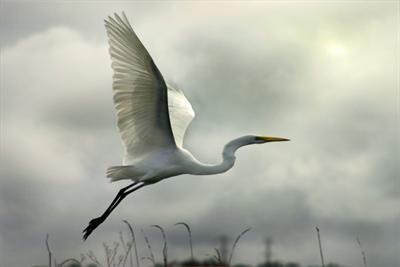
\includegraphics[width=0.72in,height=0.52in]{./MC_image/1.jpg}
    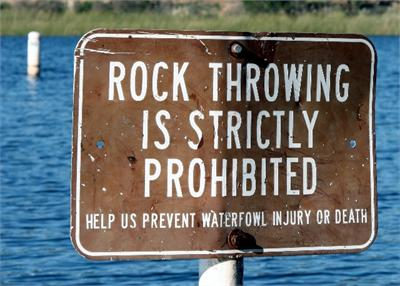
\includegraphics[width=0.72in,height=0.52in]{./MC_image/2.jpg}
    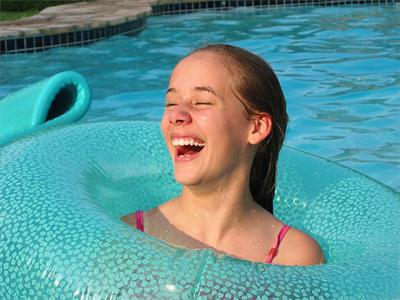
\includegraphics[width=0.72in,height=0.52in]{./MC_image/3.jpg} 
    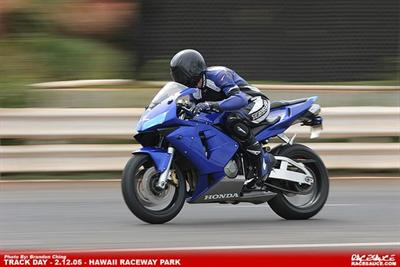
\includegraphics[width=0.72in,height=0.52in]{./MC_image/4.jpg} 
    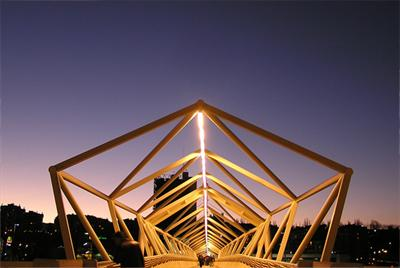
\includegraphics[width=0.72in,height=0.52in]{./MC_image/5.jpg} 
    \\
    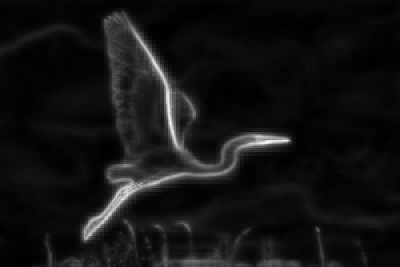
\includegraphics[width=0.72in,height=0.52in]{./MC_image/1_MC.jpg}
    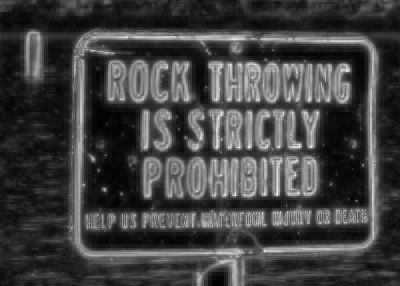
\includegraphics[width=0.72in,height=0.52in]{./MC_image/2_MC.jpg}
    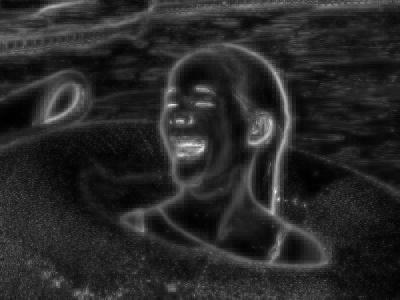
\includegraphics[width=0.72in,height=0.52in]{./MC_image/3_MC.jpg}
    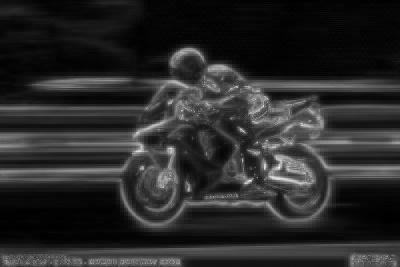
\includegraphics[width=0.72in,height=0.52in]{./MC_image/4_MC.jpg}
    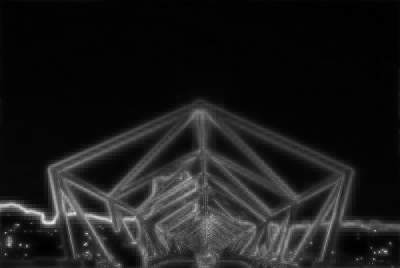
\includegraphics[width=0.72in,height=0.52in]{./MC_image/5_MC.jpg}
    \\
    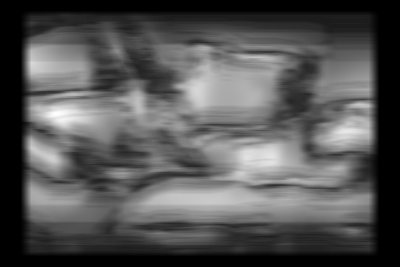
\includegraphics[width=0.72in,height=0.52in]{./MC_image/1_CSH.jpg}
    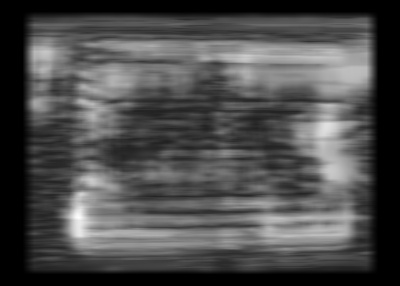
\includegraphics[width=0.72in,height=0.52in]{./MC_image/2_CSH.jpg}
    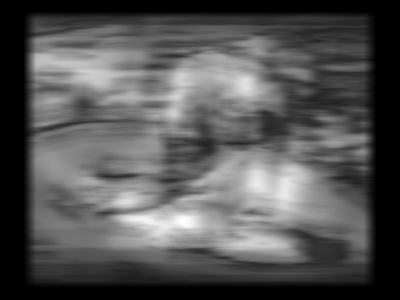
\includegraphics[width=0.72in,height=0.52in]{./MC_image/3_CSH.jpg}
    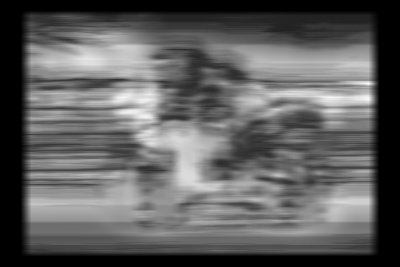
\includegraphics[width=0.72in,height=0.52in]{./MC_image/4_CSH.jpg}
    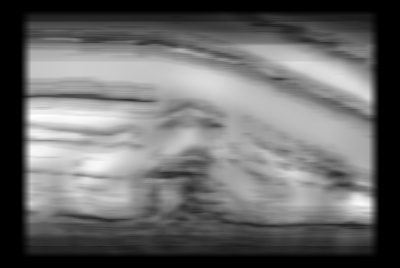
\includegraphics[width=0.72in,height=0.52in]{./MC_image/5_CSH.jpg}
    \\
    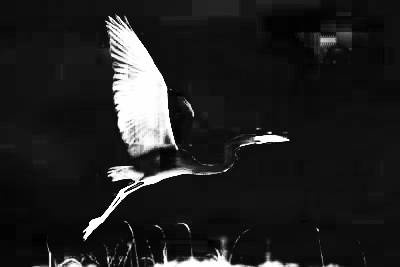
\includegraphics[width=0.72in,height=0.52in]{./MC_image/1_CSD.jpg}
    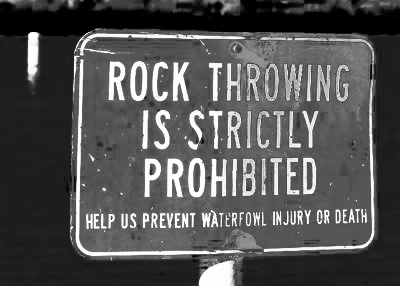
\includegraphics[width=0.72in,height=0.52in]{./MC_image/2_CSD.jpg}
    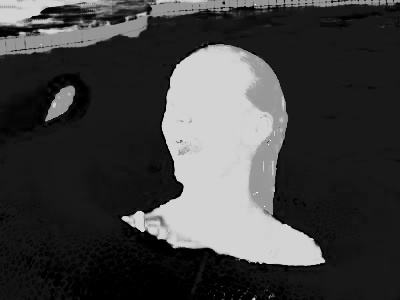
\includegraphics[width=0.72in,height=0.52in]{./MC_image/3_CSD.jpg}
    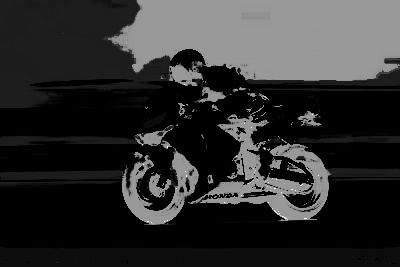
\includegraphics[width=0.72in,height=0.52in]{./MC_image/4_CSD.jpg}
    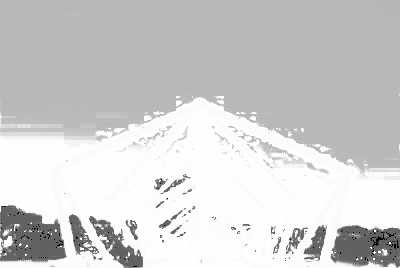
\includegraphics[width=0.72in,height=0.52in]{./MC_image/5_CSD.jpg}
\end{center}
}
\frame{
    \frametitle{Local: Multiscale Contrast}
    Create a contrast map from the linear combination of image contrast at all levels of an N-level gaussian image pyramid, using the pixels $x$ in the image $I$:
    $$
    f_c(x,I) = \SUM_{n = 1}^{N}\SUM_{x'\in W(x)}||I^n(x)-I^n(x')||^2
    $$
    where W(x) is a window that delineates which area to consider for neighbouring pixels to compare contrast values.\\[10pt]
    \begin{center}
    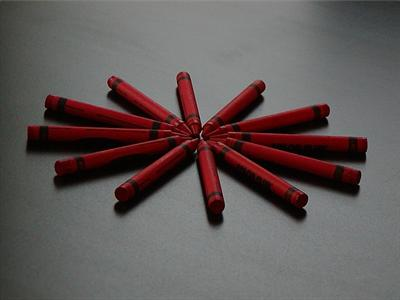
\includegraphics[width=0.72in,height=0.52in]{contrast/1orig.jpg}
    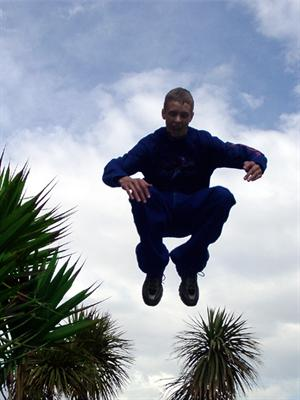
\includegraphics[width=0.72in,height=0.52in]{contrast/2orig.jpg}
    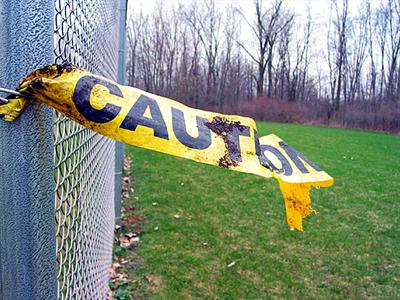
\includegraphics[width=0.72in,height=0.52in]{contrast/3orig.jpg}\\
    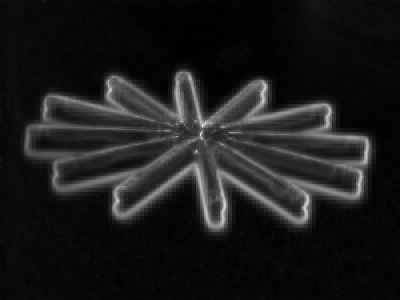
\includegraphics[width=0.72in,height=0.52in]{contrast/1cont.jpg}
    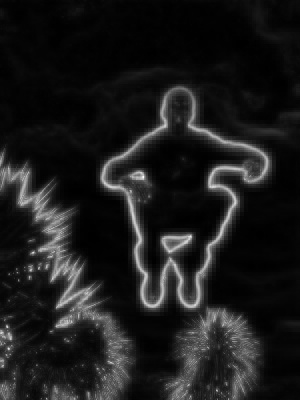
\includegraphics[width=0.72in,height=0.52in]{contrast/2cont.jpg}
    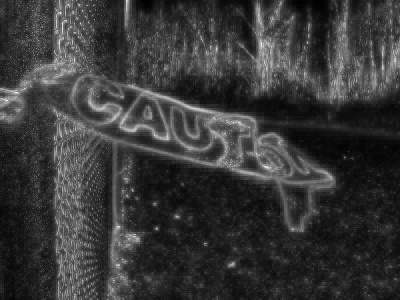
\includegraphics[width=0.72in,height=0.52in]{contrast/3cont.jpg}
    \end{center}
}
\frame{
    \frametitle{Regional: Center-Surround Histogram}
    Given a rectangle $R_s(x)$around a salient region, create a frame $R(x)$ around it so that the area of the frame is equal to that of the rectangle (this is displaced as needed to fit into the image dimensions), at a suitable aspect ratio.\\[10pt]
    PICTURES HERE.
}
\frame{
    \frametitle{Regional: Center-Surround Histogram}
    Create a colour RGB histogram for both the rectangle and the surrounding frame with a certain resolution (number of ``bins'' for each colour)\\[10pt]
%, and calculate how many pixels fall into each colour's bins in the frame and the rectangle.\\[10pt]
%    Finally, c
    Calculate the $\chi^2$ value between the two histograms to obtain the differences between the rectangle and the surrounding frame.  Do this for multiple aspect ratios, and keep the largest $\chi^2$ value: %and the frame that formed it:
    $$
    R(x) = \argmax\limits_{R(x)}\chi^2(R(x), R_s(x)) =\argmax\limits_{R(x)}\frac{1}{2}\cdot\SUM_{i\in bins}\frac{(hist_{R(x)_i}-hist_{R_s(x)_i})^2}{hist_{R(x)_i}+hist_{R_s(x)_i}}
    $$
    The center-surround histogram feature is finally calculated as:
    $$
    f_h(x,I)\propto\SUM_{x'|x\in R(x')}w_{xx'}\chi^2(R(x'),R_s(x'))
    $$

}
\frame{
    \frametitle{Global: Colour Spatial Distribution}
    
    Create a Gaussian Mixture Model to compute the spatial variance and continuity of colour in an image.\\[10pt]
    The component model is created from only a subset of the pixels in the image, and the maximum number of iterations is limited in order to reduce the time taken to compute this feature without sacrificing too much accuracy.\\[10pt]
    \begin{center}
    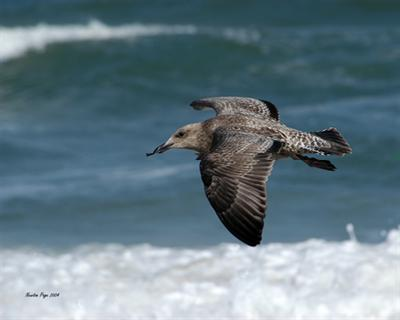
\includegraphics[width=0.72in,height=0.52in]{./CSD_image/1.jpg}
    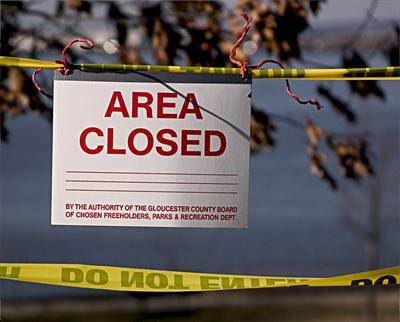
\includegraphics[width=0.72in,height=0.52in]{./CSD_image/2.jpg}
    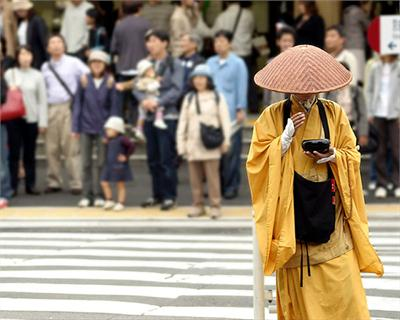
\includegraphics[width=0.72in,height=0.52in]{./CSD_image/3.jpg}\\
    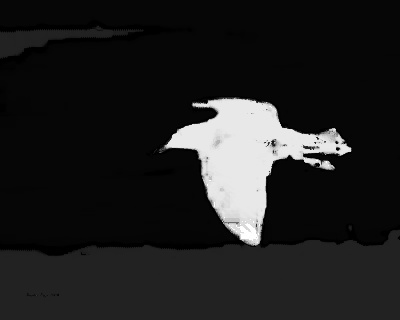
\includegraphics[width=0.72in,height=0.52in]{./CSD_image/1_CSD.jpg}
    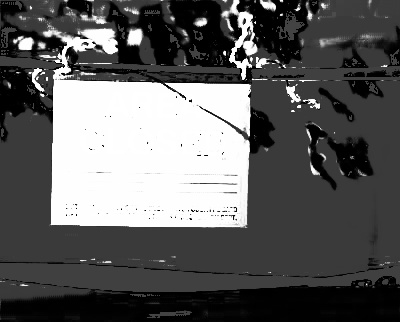
\includegraphics[width=0.72in,height=0.52in]{./CSD_image/2_CSD.jpg}
    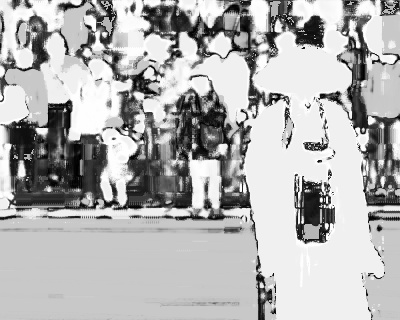
\includegraphics[width=0.72in,height=0.52in]{./CSD_image/3_CSD.jpg}
    \end{center}
}
\frame{
    \frametitle{Global: Colour Spatial Distribution}
    Each pixel is associated to a colour component with the probability
    $$
    P(c|I_x) = \frac{\omega_c\mathcal{N}(I_x|\mu_c,\sigma_c)}{\SUM_c \omega_c \mathcal{N}(I_x|\mu_c,\Sigma_c)}
    $$
    where $\omega_c$ is the weight, $\mu_c$ is the mean colour, $\sigma_c$ is the covariance, and $\mathcal N(I_x|\mu_c,\sigma_c)$ is the multivariate normal distribution of the $c^{th} component$\\[10pt]
    The final colour spatial distribution feature is defined as a weighted sum:
    $$
    f_s(x,I)\propto\SUM_c p(c|I_x)]\cdot(1-V(c))
    $$
    where $V(c)$ is the normalised covariance (horizontal and vertical variances) of the $c^{th}$ component, contained between 0 and 1.
}
%}}}

%{{{ CRF content
\section{Conditional Random Fields}
\frame{
    \frametitle{Learning}
    The values from the before-mentioned features are accumulated in a CRF model, which the dataset then trains on. MORE DETAIL HERE
}
\frame{
    \frametitle{Inference}
    CRF INFERENCE HERE
}
%}}}

%{{{ Reference
\section{References}
\frame{
    \frametitle{References}
    \begin{thebibliography}{9}
        \bibitem{ConcreteMath} Liu, Tie, et al. "Learning to detect a salient object."\textit{ Computer Vision and Pattern Recognition, 2007. CVPR'07. IEEE Conference on. IEEE, 2007. }
        \bibitem{ConcreteMath} Liu, Tie, et al. "Learning to detect a salient object."\textit{ Pattern Analysis and Machine Intelligence, IEEE Transactions on 33.2 (2011): 353-367.}
        \bibitem{ConcreteMath} Itti, Laurent, Christof Koch, and Ernst Niebur. "A model of saliency-based visual attention for rapid scene analysis."\textit{ Pattern Analysis and Machine Intelligence, IEEE Transactions on 20.11 (1998): 1254-1259.}
        \bibitem{ConcreteMath} Ma, Yu-Fei, and Hong-Jiang Zhang. "Contrast-based image attention analysis by using fuzzy growing."\textit{ Proceedings of the eleventh ACM international conference on Multimedia. ACM, 2003.} 
        \bibitem{ConcreteMath} Stephen Gould, "DARWIN: A Framework for Machine Learning and Computer Vision Research and Development", \textit{Journal of Machine Learning Research (JMLR), 13(Dec):3533−3537, 2012}.
    \end{thebibliography}
}
%}}}
\end{document}
